\documentclass[12pt]{article}
\usepackage{amsfonts, amssymb}
\usepackage{msc}
\usepackage{tikz}
	\usetikzlibrary{arrows, automata,positioning}
\usepackage{graphicx}
\usepackage{wrapfig}
\usepackage{float}
\usepackage{datetime}
\usepackage[ngerman]{babel}
\usepackage[utf8]{inputenc}
\usepackage{enumitem}
\usepackage{amsmath}
\usepackage{xspace}
\usepackage{multirow}
\usepackage{mathtools}
\usepackage{hyperref}

\newdateformat{specialdate}{\twodigit{\THEDAY}.\twodigit{\THEMONTH}.\THEYEAR}

\newcommand{\blue}[1]{\color{blue}#1\color{black}\xspace}
\newcommand{\red}[1]{\color{red}#1\color{black}\xspace}
\newcommand{\green}[1]{\color{green}#1\color{black}\xspace}

\makeatletter
\newcommand*\bigcdot{\mathpalette\bigcdot@{.5}}
\newcommand*\bigcdot@[2]{\mathbin{\vcenter{\hbox{\scalebox{#2}{$\m@th#1\bullet$}}}}}
\makeatother


\begin{document}
	
	\title{MAO - Zusammenfassung}
	\author{Timo Bergerbusch}
	\date{\specialdate\today}
	\maketitle
	
	\tableofcontents
	\newpage
	
	\section{Typische Probleme} \label{Standard Probleme}
		\subsection{Matching}
			Paarbildung von adjazenten Knoten in einem ungerichteten bewerteten Graphen\\
			Matching $M$: jeder Knoten hat max. einen Partner Knoten\\
			perfektes Matching $M^*$: jeder Knoten hat genau einen Partner Knoten\\
			Optional: Kosten, Profite, etc\dots
		\subsection{Set-Packing/Covering/Partitioning}
			\subsubsection*{Gegeben: }
			\begin{itemize}
				\item $m$-elementige Menge $M={1, \dots, m}$
				\item $n$ Teilmengen $M_1,\dots,M_n \subset M$
				\item Kosten/Profite der Teilmengen $c_1,\dots,c_n$
			\end{itemize}
			\subsubsection*{Gesucht:} Auswahl von Teilmengen
			\begin{enumerate}
				\item mit max. Profit / min. Kosten
				\item die Grundmenge $M$ wird gepackt, überdeckt oder partitioniert
			\end{enumerate}			
			Eine Lösung $L$ ist ein
			\begin{itemize}
				\item Set-Packing, wenn $M_j \cap M_k = \emptyset \forall j,k \in L, j \neq k$
				\item Set-Covering, wenn $\bigcup_{j\in L} M_j = M$
				\item Set-Partitioning, wenn es sowohl Set-Packing als auch Set-Covering ist
			\end{itemize}
		\subsection{Traveling-Salesman-Problem (TSP)}\label{TSP}
			\subsubsection*{Gegeben:}
			\begin{itemize}
				\item vollständiger Graph $G=(V,E,d)$
				\item symmetrisch: $d_{i,j}=d_{j,i}\> \forall i,j\in V$
				\item asymmetrisch: $d_{i,j}\neq d_{j,i}\> \exists i,j \in V$
			\end{itemize}
			\subsubsection*{Gesucht:}
			kostenminimale Hamilton-Tour
			
			\subsubsection{Typische Distanzmatrixberechnung:}
			Euklidische Distanz: $d_{i,j}=\sqrt{(x_i-x_j)^2+(y_i-y_j)^2}$ \\
			Manhattan-Distanz: $d_{i,j}=|x_i-x_j|+|y_i+y_j|$
		\subsection{Bin-Packing-Problem (BPP)}
			\subsubsection*{Gegeben:}
				\begin{itemize}
					\item Kapazität $C>0$
					\item Gewichte $w_1,\dots,w_n$ mit $0<w_i\le C$
				\end{itemize}
			\subsubsection*{Gesucht:}
				Partitionierung $P_1\cup\dots\cup P_k = \{1,\dots,n\}$ mit $P_i\cap P_j = \emptyset$ und $\sum_{j\in P_i} w_j \le C$ für ein minimales $k$.

			\subsubsection*{Greedy-Algorithmus}\label{BPGreedy}
			Unterscheide die versch. Strategien
			\begin{itemize}
				\item Weight Decreasing: absteigend nach Gewicht sortiert
				\item Next-Fit: Zuordnung zum zuletzt geöffneten
				\item First-Fit: Zuordnung zumersten geöffneten Behälter mit kleinstem Index
				\item Best-Fit: Zuordnung zum Behälter mit kleinster noch ausreichender Kapazität
			\end{itemize}
		
		\subsection{Rucksackproblem (KP)}
			\subsubsection*{Gegeben:}
			\begin{itemize}
				\item Rucksack mit Kapazität $C$
				\item $n$ Gegenstände mit Gewicht $w_i$ und Profit $p_i$
			\end{itemize}
			
			\subsubsection*{Gesucht:}
			Profit-maximale Teilmenge von Gegenständen, welche nicht schwerer ist als $C$
			
			\subsubsection*{Greedy-Algorithmus}\label{KPGreedy}
			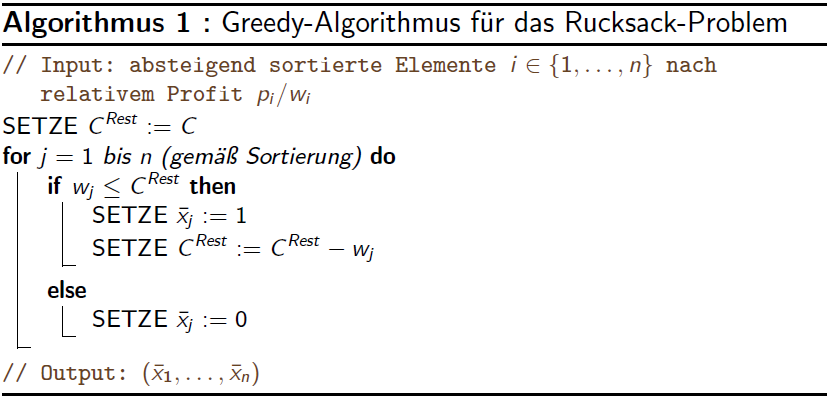
\includegraphics[scale=0.6]{KPGreedy}
	\section{1. Kapitel - Einführung}
	\begin{itemize}
		\item Abgrenzung Modell und Methode:
			\begin{itemize}
				\item[Modell:] modellieren, darstellen, abbilden
				\item[Methode:] rechnen, Algorithmus
			\end{itemize}
		\item Beispielanwendungen:
			\begin{itemize}
				\item Demand Planning: Welche Dienstleistungen auf welchen Flugstrecken
				\item Umlaufplanung: Welches Flugzeug für welchen Flug?
				\item Crew Scheduling: Wer erledigt wann welche Aufgaben?
				\item Disruption Management: Wie reagieren auf Störungen, Abweichungen und Ausfälle?
				\item Revenue Management: Pricing, Kapazitätssteuerung
				\item Netzwerk-Design: Welche Standorte und welche Aufgaben dort?
				\item Transportplanung
				\item Standort Planung
				\item "Letzte Meile": Bezirkseinteilung und Postbotenrouten
			\end{itemize}
		\item \textbf{optimal} \label{optimal}\label{Optimum}: zulässig und bestmöglich
		\item \textbf{Simulation} \label{Simulation}: Durchführung von Experimenten anhand von Modellen
		\item Optimierung:
			\begin{itemize}
				\item exakt vs. heuristisch
				\item kontinuierlich vs. diskret
				\item linear vs. nicht-linear 
			\end{itemize}
		\item \hyperref[Simulation]{Simulation} vs. Optimierung:
			\begin{itemize}
				\item Simulation zeigt nur Konsequenzen von Entscheidungen auf
				\item Simulation macht keinen Entscheidungsvorschlag
				\item Simulation gestattet nur den Vergleich von Alternativen
			\end{itemize}		
		\item \textbf{Heuristik} \label{Heuristik}: 
			\begin{itemize}
				\item[Def.:] Algorithmen die ein geg. Optimierungsproblem mit akzeptablem Aufwand in möglichst gut zu lösen versuchen
				\item[Kennzeichen:] Ausschluss potentieller Lösungen, fehlende Lösungsgarantie, nicht-willkürliche Lösungssuche(, künstliche Stoppregel)
				\item[Prinzipien] Allgemeinheit, Effizienz, Optimalität	\\
				\begin{tikzpicture}
				\node[rectangle, draw, rounded corners] (allg) {Allgemeinheit};
				\node[rectangle, draw, rounded corners, below right = 3cm of allg] (opt) {Optimalität};
				\node[rectangle, draw, rounded corners, above right = 3cm of opt] (eff) {Effizienz};
				
				\path[thick]
				(allg) edge node[sloped, align = left] {exaktes\\ Verfahren} (opt)
				(allg) edge node[anchor=south] {Heuristik} (eff)
				(opt) edge node[sloped, align = left] {Verfahren für \\ spez. Instanz} (eff);
				\end{tikzpicture}
				\item[Klassifikation] nach Stopp-Regel:
				\begin{enumerate}
					\item[Eröffnungsv.] generieren einer (mögl. guten) Lösung. Terminierung sobald Lösung gefunden
					\item[Verbesserungsv.] Start mit zulässiger Lösung und verbessern, bis Stopp-Krit. erfüllt ist
					\item[Zsm.-gesezte V.] Kombination von Eröffnungs- und Verbesserungsv.
				\end{enumerate} 
			\end{itemize}
		\item \textbf{Algorithmus} \label{Algorithmus}: 
			\begin{itemize}
				\item[Def.:] Ein Algorithmus ist eine genau definierte Verarbeitungsvorschrift zur Lösung eines Problems oder einer bestimmten Art von Problemen. Typischerweise wird ein Algorithmus durch eine endliche Folge von Anweisungen beschrieben, die nacheinander ausgeführt und oft in festgelegter Weise wiederholt werden
				\item[Eig.:] eindeutig, allgemein, ausführbar, endlich
			\end{itemize}
		\item \textbf{exakter Algorithmus} \label{exakter Algorithmus}: ein \hyperref[Algorithmus]{Algorithmus}, welcher für jede Instanz
			eines Optimierungsproblems ein \hyperref[Optimum]{Optimum} bestimmt
		\item \textbf{Laufzeitkomplexität}: \hyperref[Algorithmus]{Alg. A} ist in $\mathcal{O}(f(n)) \text{, gdw } \exists k_1,k_2$ konst.,
			sodass $\text{time}_A(P) \le k_1+k_2 f(n)$ für alle Instanzen $P$ mit $|P|=n$
		\item \textbf{effizienter Algorithmus} \label{effizienter Algorithmus}: A ist effizient gdw $A \in \mathcal{O}(f(n))$
		\item \textbf{$\mathcal{P}$} \label{P}: alle Probleme mit einem deterministischen 
			\hyperref[effizienter Algorithmus]{effizienten Algorithmus}.
		\item \textbf{$\mathcal{NP}$} \label{NP}: alle Probleme mit einem nicht-deterministischen
			\hyperref[effizienter Algorithmus]{effizienten Algorithmus}.
		\item \textbf{polynomiale Reduzierbarkeit}\label{polyRed}: 
			Geg.: Probleme $\Pi_1, \Pi_2$, Funktionen $f:\Pi_2\rightarrow\Pi_1$ und $g:L(\Pi_1)\rightarrow L(\Pi_2)$\\
			$\Pi_2$ ist polynomial reduzierbar auf $\Pi_1$, gdw. $f$ und $g$ polynomial berechenbar sind
		\item \textbf{$\mathcal{NP}$-schwer} \label{NPschwer}: falls jedes $\Pi'\in\mathcal{NP}$ \hyperref[polyRed]{pol. red.} auf $\Pi$ ist
		\item \textbf{$\mathcal{NP}$-Vollständig} \label{NPvoll}: falls $\Pi$ $\mathcal{NP}$-schwer und $\Pi\in\mathcal{NP}$
	\end{itemize}

	\section{2. Kapitel - Greedy Algorithmen}
		\begin{itemize}
			\item \textbf{Greedy-Algorithmus} \label{greedy}: Greedy = gierig; Greedy-Prinzip: fixiere Variable die jetzt die größte Verbesserung darstellt\\
			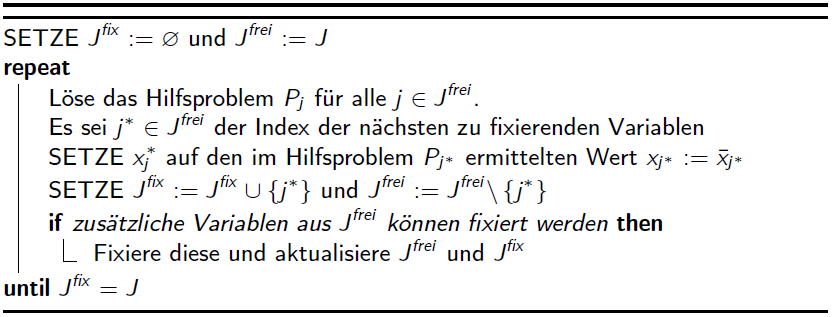
\includegraphics[scale =0.6]{AllgGreedy}
			\item Eröffnungsverfahren
			\item \hyperref[BPGreedy]{BPP-Greedy} und \hyperref[KPGreedy]{KP-Greedy}
			\item MST-Greedy Algorithmus: \\
				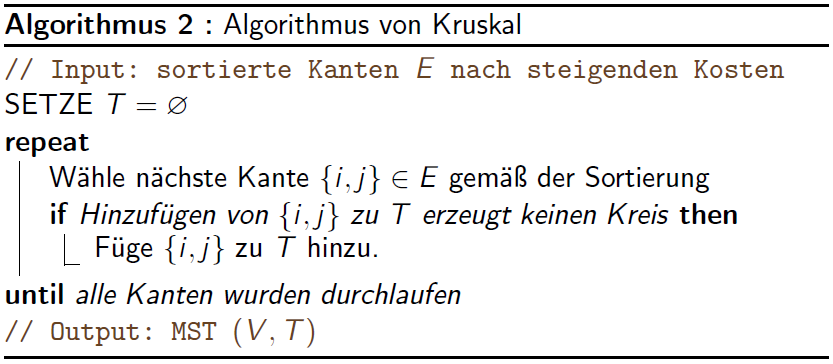
\includegraphics[scale=0.6]{KruskalGreedy}
			\item meinst \underline{nicht} optimal
			\item Nutzenmöglichkeit: \begin{enumerate}
					\item unzulässige Lösungen zulassen und mit Strafkosten versehen
					\item Wiederholen mit mod. Kosten/Koeffizienten/(Ersatz-)Problem
				\end{enumerate}
		\end{itemize}
	\section{3. Kapitel - Lösungsqualität und Approximation}
		\begin{itemize}
			\item\textbf{Performance-Verhältnis} \label{Performance Verhaeltnis}: Probleminstanz $P\in \Pi$, Heuristik \\ 
				$H \Rightarrow R_H(P)=\frac{z_H(P)}{z_{opt}(P)}$ 
			\item wenn Performance Verhältnis = 1 für alle Instanzen von $P$ $\Rightarrow$ exakter Opt.-Algo.
				\begin{itemize}
					\item Minimierungsproblem: $R_H(P) \ge 1$
					\item Maximierungsproblem: $R_H(P) \le 1$
				\end{itemize}
			\item \textbf{Performance Analysen}\label{Performance Analyse}:
				\begin{itemize}
					\item[worst-case:] schlechtestes Performance Verhältnis
					\item[average-case:] durchschnittliches Performance Verhältnis über \underline{alle} Instanzen, via Wahrscheinlichkeitsverteilung, Erwartungswert und Varianz
					\item[empirisch:] durchschnittliches Performance Verhältnis, maximale Abweichung und empirische Varianz über \underline{relevante} Instanzen
				\end{itemize}
			\item \textbf{$\epsilon$-Approximationsalgorithmus}\label{eApproxAlgo}: Für $\epsilon\ge 0$, Heuristik $H$. $H$ ist $\epsilon$-Approximationsalgorithmus gdw.
				\begin{itemize}
					\item $R_H \le 1- \epsilon$, für Minimierungsp.
					\item $R_H \ge 1- \epsilon$, für Maximierungsp.
				\end{itemize}
		\end{itemize}
	\section{4. Kapitel - Lokale Suche}
		\begin{itemize}
			\item Grundidee: geg. zulässige Lösung in eine andere bessere zulässige Lösung transformieren und rekursiv wiederholen
			\item \textbf{Nachbarschaft} \label{Nachbarschaft}: Abbildung $ \mathcal{N}:X\rightarrow Pot(X)$
			\item \textbf{verbessernder Nachbar} \label{verbessernder Nachbar}: zu min. Ziel-fkt $z$: $x'\in\mathcal{N}(X)$ mit $z(x')<z(x)$ heißt verbessernder Nachbar
			\item \hyperref[Nachbarschaft]{Nachbarschaften}, \hyperref[verbessernder Nachbar]{Nachbarn}
			\item Pseudocode:\\
				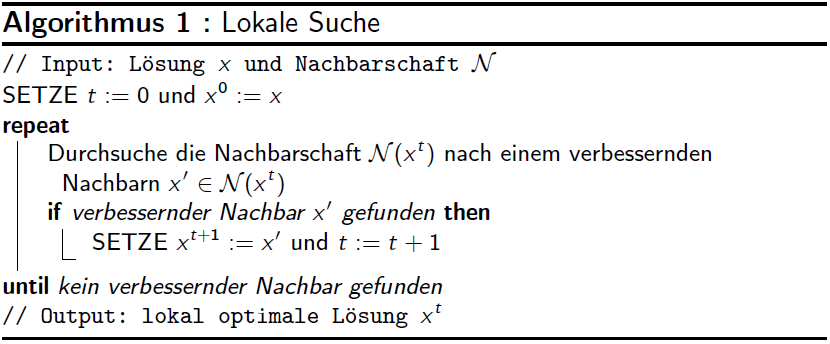
\includegraphics[scale=0.6]{LokaleSuche}
			\item Suchstrategien:
				\begin{itemize}
					\item[Erstensuche:] suche ersten \hyperref[verbessernder Nachbar]{verbessernden Nachbarn}
					\item[Bestensuche:] suche besten \hyperref[verbessernder Nachbar]{Nachbarn}
					\item[$l$-Erstensuche:] suche ersten $l$ \hyperref[verbessernder Nachbar]{verbessernde Nachbarn}
				\end{itemize}
			\item 2-Opt Nachbarschaft:
				\begin{itemize}
					\item Für (S)\hyperref[TSP]{TSP}: Entfernen von 2 nicht benachbarten Kanten und hinzufügen von zwei anderen
					\item $n$-Städte: $|\mathcal{N}_{2Opt}(X)|= \frac{n(n-3)}{2}$
				\end{itemize}
			\item \textbf{Nachbarschaftsgraph} \label{Nachbarschaftgraph}: $(X,A_\mathcal{N})$ mit $X$ alle zulässigen Lösungen, $(x,x')\in A_\mathcal{N}$, falls $x'\in\mathcal{N}(x)$
			\item \textbf{stark Zusammenhängend} \label{starker Zusammenhang}: Falls von jeder Lösung $x,y\in X$ ein Weg $\pi$ ex., sodass $\pi= x\dots y$
			\item \textbf{Transitionsgraph} \label{Transitionsgraph}: $(X,A_\mathcal{N}^{trans})$ mit $X$ alle zulässigen Lösungen, $(x,x')\in A_\mathcal{N}$, falls $x'$ ein \hyperref[verbessernder Nachbar]{verbessernder Nachbar} von $x$ ist
			\item \textbf{exakte Nachbarschaft}\label{exakte Nachbarschaft}: Wenn jedes lokale Optimum auch ein globales Optimum ist
			\item \textbf{Durchmesser einer Nachbarschaft}\label{Durchmesser}: max. Länge eines kürzesten Weges
			\item Wünschenswerte Eigenschaften:
				\begin{enumerate}
					\item \hyperref[starker Zusammenhang]{starker Zusammenhang}
					\item Symmetrie: $x\in\mathcal{N}(x') \Leftrightarrow x\in\mathcal{N}(x')$
					\item Effiziente Berechnung des Zielfunktionswertes.
					\item Effiziente Konstruktion von $\mathcal{N}$
					\item Effiziente Zulässigkeitsprüfung
					\item Effiziente Suche nach \hyperref[verbessernder Nachbar]{verbessernden Nachbarn}
				\end{enumerate}
			\item \textbf{Sequentielle Suche}\label{sequentielle Suche}:
				\begin{itemize}
					\item[Idee:] Lösche $(x,x')$ $\rightarrow$ Füge $(x',x'')$ hinzu $\rightarrow$ Lösche $(x'',x''')$ $\rightarrow$ \dots
					\item[In 2-Opt:] $t_1,t_2,t_3,t_4$, wobei $(t_1,t_2)$ und $(t_3,t_4)$ gelöscht und $(t_2,t_3)$ und $(t_1,t_4)$ hinzu gefügt wurden
					\item[$\Rightarrow$] für $g_1 = c_{t_1,t_2}-c_{t_2,t_3}$ und $g_2= c_{t_3,t_4}-c_{t_4,t_1}$ will man $g_1+g_2 > 0$ für Verbesserung
					\item[$\Rightarrow$] man genötigt $g_1 > 0$ und $g_1+g_2 > 0$ (einer muss $>0$ sein und wenn $g_1+g_2 > 0$ und $g_1\le0$ dann stimmt die Aussage für $g_1'=g_2$ und $g_2'=g_1$)
					\item Algorithmus:\\
						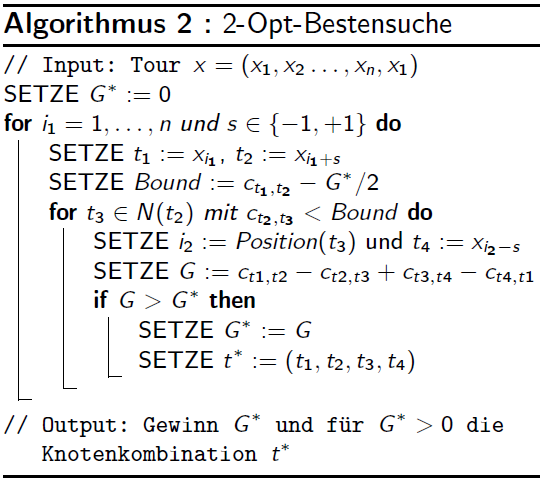
\includegraphics[scale=0.6]{SequentielleSucheAlgo}\\
						(Wichtig: \texttt{bound} fängt den symmetrischen Fall ab und bedeutet soviel wie: wir müssen bereits mit der ersten Löschung min. die Hälfte der Einsparung machen)
				\end{itemize}
		\end{itemize}
\end{document}